\documentclass{article}


\usepackage[a4paper]{geometry}
\usepackage{graphicx}


\begin{document}
\date{} 
\section{\bf Calorimeter R\&D}

\subsection{Silicon-Tungsten ECAL in ILD}
\subsubsection{Introduction}

The group of the silicon-tungsten electromagnetic calorimeter for ILD aims to develop a highly
granular detector optimized for particle flow measurements. The calorimeter uses a
sandwich architecture of silicon sensors with 5$\times$5 mm$^2$ pixels as active elements embedded in an
alveolar structure made of tungsten and carbon fiber. The group is active in the development of simu-
lation software and algorithms for calorimeter reconstruction, as well as in the design of readout
chips, front-end electronics boards, mecanical structures, cooling and in ILD 
integration.

\subsubsection{Recent Milestones}

The work is now focusing on the construction of a technological prototype. This
is a new milestone after the successful operation of the “Physics Prototype” in the
years 2004-–2011, including large scale beam tests at DESY, CERN and FNAL and data
analysis~\cite{physprot}.

In the technological prototype and in the ILD design the front end SKIROC
chips~\cite{skiroc} are embedded into the calorimeter layers and mounted on
multi-layer printed circuit boards (PCBs). Four silicon sensors are glued with
a conductive epoxy to the readout PCB. Depending on the ILD and the silicon
sensor sizes, up to about ten of these PCBs will be connected together in-line
and read out from one end by a data acquisition (DAQ) electronics. The sandwich
of the silicon sensors with PCBs on both sides of the absorber layer
represents one active module, called ``slab''. It is slided in the tungsten --
carbon fiber alveolar structure. The slab absorber layer is also made of
tungsten wrapped in carbon fiber. In this way, half of the absorber layers are
in the structure and half are in the slabs.

A series of tests with simplified PCBs have been carried out starting from
2012: several beam tests at DESY, cosmic calibrations and infrared laser
tests. Each simplified PCB served one silicon sensor.  The power pulsing
operation of the SKIROC chips has been demonstrated. The bias currents of the
chips were shut down and raised with a frequency between 1 -- 20~Hz.  It was
shown that the SKIROC currents should be switched on at least 600~$\mu$sec
before physical events, so that all transition processes are finished.
Mechanical rigidity of electrical interconnections under changing Lorentz
force and also, the stability of pedestals was checked in the power pulsing
mode in the magnetic fields of up to 2 T.  The continuous cosmic data taking
during 24 hours allowed to calibrate each pixel with 3\% statistical accuracy.
The variation of cosmic MIP signals across all channels was measured at 3-4\%
level.  It was found to be dominated by the spread between the chips and by
the variation of electronic channel gains within a chip. The same spread is
measured by a calibrated charge injection into SKIROC preamplifiers.  In
cosmic and test beam data the signal-over-noise ratio for MIP signals was
measured at the level of 8 -- 20. It depended on the SKIROC gain, the better
values were obtained for the gain 5 times higher than nominal.

The infrared laser tests have been used to study the so-called ``square''
events. They are caused by a capacitive coupling (cross-talk) between a
silicon sensor guard ring and its boundary pixels. The guard ring ensures low
dark currents of the sensor under high voltage. For technological reasons it
is not grounded. High local signals at the sensor periphery may, therefore,
propagate to all boundary pixels, fire them and produce ``square''
events. With an improved segmented guard ring design, the cross-talk is
reduced to $\le$0.5\% per outer pixel side, as it was measured with the laser
induced signals. Hamamatsu HPK company also developed a new ``no guard ring''
design, their small sensors demonstrated both the lowest guard ring
cross-talks and sufficiently low dark currents. Another activity which has
been started in 2015, is the study of dark current dependence on neutron
irradiation dose at a nuclear reactor.

Generally, the analysis of accumulated beam test, cosmic and infrared laser
data validated the concept of the front end electronics. It will also allow
for correcting an observed shortcomings of the SKIROC chips and the first
PCB. A new version of PCB serving four sensors as required for ILD, has been
designed and produced, see Fig.~\ref{ild_siw_ecal_fev}.
\begin{figure}
\centering
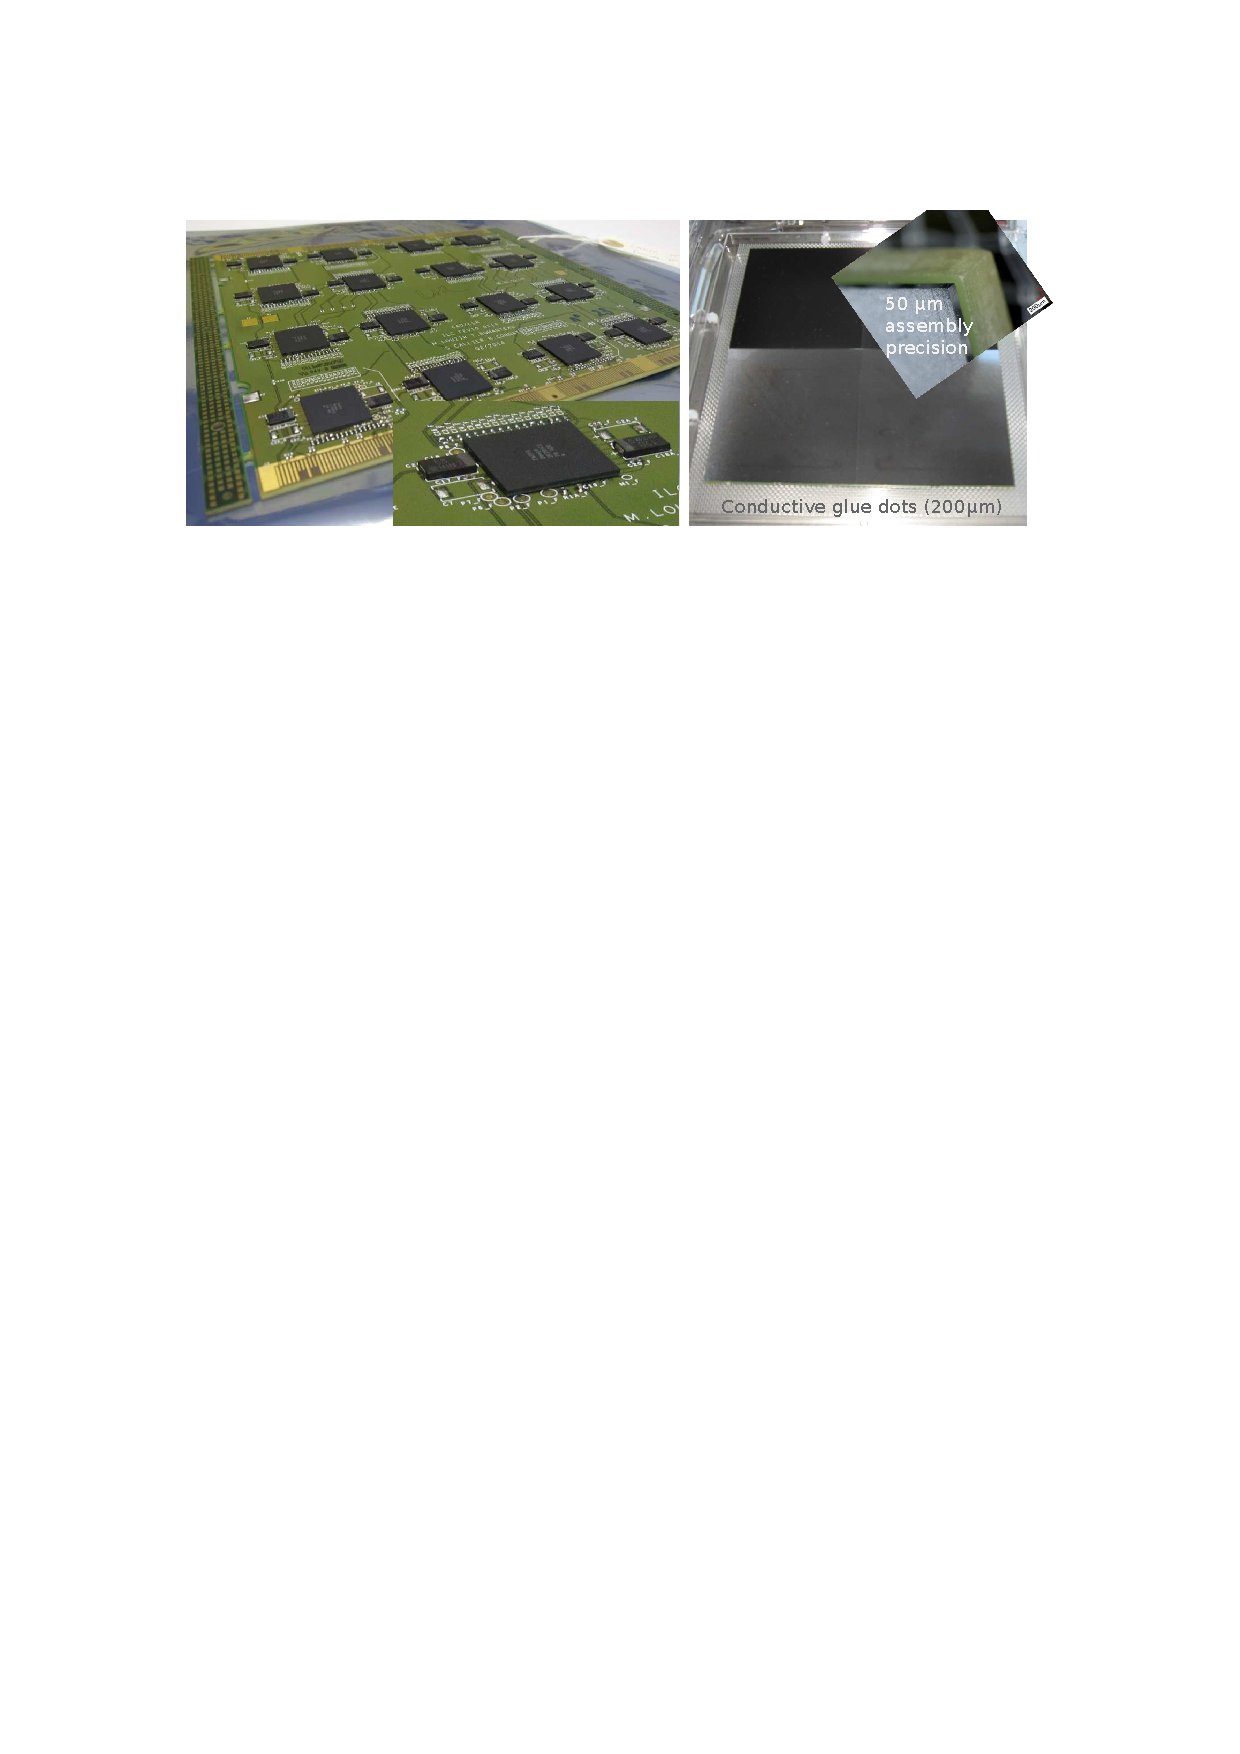
\includegraphics[width=\textwidth]{FEV_gluing_photo.pdf}
\caption{Left: new PCB with 16 SKIROC chips and 1024 channels, right: 4 sensors
  aligned and prepared for robotic gluing to PCB.}
\label{ild_siw_ecal_fev}
\end{figure}
To increase a channel density, a ball grid array
(BGA) packaging of the SKIROC chips was chosen. The gluing of four fragile silicon
sensors with a gap in between of only 100 $\mu$m has been successfully
performed with a robot. The first detectors have been assembled in 2015 and
the first tests with the cosmics and the laser have shown a good performance. An assembly
procedure together with quality controls is formalized and well documented.
Further improvement and production of the new version of SKIROC chips is planned
for both ILD and for a CMS phase-2 endcap calorimeter upgrade project
(HGCAL). The combined with HGCAL beam tests at SPS in CERN are planned in
November 2015 and in 2016.

The mechanical design of ILD ECAL is well advanced. A full scale prototype of
a barrel tungsten -- carbon fiber alveolar module with three towers of 15
alveoli has been successfully produced with required tolerances. A full scale
absorber part of the barrel slab has been also manufactured with tungsten
substituted by carbon to reduce the cost. The mechanical simulations of one
alveolus structure have been verified with the measurements using a special
prototype with molded Bragg grating fibers. When elongated under loads, such
fibers change a frequency of reflected light, allowing very precise
measurements. The same technique is used in constructing buildings, bridges
etc.  A long 2.5~m endcap carbon structure with 3 alveoli is also
successfully produced. The rails supporting ECAL on the HCAL face in ILD, and
also the transport and handling tools for future ECAL assembly have been
designed and mechanically simulated.

Thermal simulations have shown that a passive cooling inside alveoli should be
sufficient. Outside water cooling will be performed with leakless loops, first
prototypes exist.

In addition to the hardware development, there is a big activity on ILD
optimization and on PFA algorithms. In particular, it was shown that the big
ILD ECAL with fine longitudinal segmentation which was chosen in DBD on the
basis of a physical performance, may be not optimal in terms of a cost
effectiveness~\cite{smallild}. In particular, the number of ECAL layers may be
reduced, eg. 19 layers provide only $\le$10\% worse jet energy resolution than
the nominal 29. Even bigger cost savings may be achieved by reducing ECAL
sizes. Eg. with an inner ECAL radius of 1400~mm instead of the nominal 1843~mm
and a proportional reduction of an ECAL length, the 45--250~GeV jet energy
resolution is degraded by 8--19\%. It may be partially compensated by an
increase in a magnetic field. In addition to the jet resolution, the
performance of a smaller ILD for a reconstruction of tau decay modes has been
studied~\cite{trantau}. It is essential for a measurement of CP-violation in
$H^0\to \tau^+\tau^-$ Higgs decays, where $\tau$ polarization is extracted
from its decay products. It was shown, that the $\tau$ mode reconstruction
efficiencies change by $\le$1\% when the ECAL radius is reduced to 1450~mm and
the magnetic field is increased from 3.5 to 4~T. Based on these studies and
taking into account the ECAL silicon sensor size, two new ILD models have been
proposed for ILD community~\cite{henrimodels}, with the ECAL inner radii of
1615 (``Khephren'') and 1480~mm (``Mykerinos'', by the name of the third
ancient Egyptian pyramid). The ECAL engineering models for these sizes are
under development.

Another important activity is a continuous improvement of PFA programs
GARLIC~\cite{garlic} and ARBOR~\cite{arbor}. The former is specialized on a
photon reconstruction in the highly granular ECAL, the latter is a PFA program
approaching PANDORA~\cite{pandora} in performance. Both programs are under
active development.

A shower fractal dimension measured in the highly granular calorimeter has
been studied in~\cite{fractal}. It was demonstrated, in particular, that the
fractal dimension could be effectively used to distinguish electromagnetic and
hadronic showers. The performance of PANDORA, ARBOR and GARLIC to separate two
electromagnetic or electromagnetic -- hadronic showers is being verified with
the physical prototype data collected in 2007 -- 2011. Such a separation is
crucial for reducing a PFA confusion. A good agreement between Monte Carlo and
data has been observed. In another analysis, a detailed study of hadronic
interactions recorded in ECAL physical prototype has been compared with GEANT4
models~\cite{naomi}.

PANDORA jet energy resolution has been studied in DBD geometry~\cite{tokyo} as
a function of several ECAL parameters, including PCB thickness, guard ring
size and fraction of dead channels and chips. It was demonstrated that the PCB
thickness with BGA packaging already achieved in the technological prototype
is sufficiently small (about $\sim$3\% degradation of jet energy resolution
compared to zero thickness). The standard guard ring thickness of 500~$\mu$m
is also sufficiently small (1-2\% degradation compared to zero). The
dependence on the fraction of randomly distributed dead channels is rather
weak, even at 10\% the jet energy resolution degrades by $\le$4\%.

\subsubsection{Plans for the near future}

The ILD slab has on each side several PCBs connected in-line. Both supply
voltages, clock and readout signals should be well propagated along the slab
through the PCBs and interconnections between them.  The assembly of in-line
PCBs partially equipped with sensors (at least at the ends) is an important
R\&D activity for the future.  For this purpose, we plan to develop an
assembly line, incorporating the reception and the test of the material, the
alignment of the PCBs, sensors and the interconnections, with a continuous
monitoring for quality control purposes. First, a manual assembly line capable
for a small production will be realized. Based on it, we will propose an
automatized system for mass assembly together with industrial partners. A
survey to search for such partners is a part of the proposal. A goal is to
design the system such that it can be duplicated at other sites.

When built, the long slab will be tested at beams and with cosmics. The
detailed characterization of channel responses will be obtained with the
calibrated charge injection. A special study of various types of cross-talks
is foreseen (across channels of one SKIROC chip, especially in high occupancy
events, noise pick-up from PCB digital lines etc.).

Like this was done for the ECAL physical prototype, we plan common beams with
other CALICE calorimeters, when our DAQ systems are sufficiently well
integrated to acquire common data.

Hamamatsu HPK produces sensors from 6 inches wafers with the typical
thicknesses in the range 300--500~$\mu$m. Another company, LFoundry in Europe,
may produce in large scale the sensors from 8 inches wafers with the thickness
of about 700~$\mu$m. Larger sensors have less fraction of guard ring dead
area, while thicker sensors provide slightly better ECAL photon
resolution. The LFoundry sensors which have been already ordered, will be
tested in the future.  In parallel, the tests of existing Hamamatsu prototypes
will continue, in particular, the cross-talk studies with the infrared laser
and the neutron irradiation measurements. The radiation hardness measurements
of other slab components is also planned. The sensors from other companies
(not only Hamamatsu) may also be tested in the same way. One may expect a
future growth of a market of large area silicon detectors due to a future mass
production of sensors for CMS HGCAL.

Other ECAL R\&D may also greatly benefit from the synergy with the HGCAL
project. It is expected that a new improved version of SKIROC chip will be
manufactured for both HGCAL beam tests and for ILD. After that, when the
SKIROC performance is proved to be sufficiently stable, a new chip generation
will be designed and produced which will have zero (pedestal) suppression.
Alternatively, if a new chip with superior characteristics will be developed
for CMS HGCAL, it may be tested and adapted for ILD purposes (note, that HGCAL
does not have the power pulsing and its bunch spacing is 25~nsec).

A continuous development of DAQ electronics is another important
activity. In addition to the optimization of the baseline PCB with BGA
packaging which should at least closely follow the SKIROC development, there
is a R\&D on embedding naked dye SKIROC chips inside the PCB. This option may
provide $\sim$1.5~mm thinner active ECAL layer, but is technologically
challenging because of the constraints on the required PCB flatness. Further
R\&D on improvement and miniaturization of DAQ electronics placed at the end
of the slab, and also, on low and high voltage distribution systems is also
foreseen.

All activities mentioned above also imply the search for industrial partners
where the future mass production may be realized. This also means a continuous
work on a cost estimation and optimization of all ECAL elements.

The work on physics -- cost optimization of ILD ECAL will continue, together
with the optimization of PFA algorithms. ECAL endcap ring should be designed
taking into account high backgrounds closer to the beam pipe. The questions of
ECAL integration in ILD, its assembly and safety will be further elaborated. 

\subsubsection{Engineering Challenges}

The following challenges will have to be addressed when proposing this
technology for ILD:
\begin{itemize}
\item cost reduction of calorimetric silicon sensors, direct contact
  with producers is already established (Hamamatsu, LFoundry, On-Semi, $\ldots$).
\item A chip with the good trigger stability, dynamic range, low noise and
  power dissipation, power pulsing etc.
\item Integration in a compact device, satisfying all the requirements
  (mechanical tolerances, readout signal quality, heat dissipation / cooling,
  reliability).
\item Industrialization of solutions, scalability of all elements for O(10M)
  or 100M channel detector.
\end{itemize}


\subsubsection{Applications Outside of Linear Colliders}
\begin{itemize}
\item CMS phase-2 upgrade project of the
  endcap calorimetry (HGCAL).
\item The compact Silicon-W design has been used in the PAMELA satellite (very
  similar to the CALICE SiW ECAL physics prototype)~\cite{pamela}.
\item Future circular $e^+e^-$ high energy colliders (FCC in CERN, CEPC in China) 
may also use this technology.
\end{itemize}

\begin{thebibliography}{1}
\bibitem{physprot} CALICE collaboration, J.~Repond {\it et al.}, ``Design and electronics
  commissioning of the physics prototype of a Si-W electromagnetic calorimeter
  for the International Linear Collider'', J. Instr. {\bf 3} (2008) P08001; arXiv:0805.4833v1 (physics.ins-det);\\
CALICE collaboration, C.~Adloff {\it et al.}, ``Response of the CALICE Si-W
electromagnetic calorimeter physics prototype to electrons'', Nucl. Instrum.
Meth. {\bf A608} (2009), 372; arXiv:0811.2354 (physics.ins-det);\\
CALICE collaboration, C.~Adloff {\it et al.}, ``Study of the interactions of pions in
the CALICE silicon-tungsten calorimeter prototype'',
J. Instr. {\bf 5} (2010) P05007; arXiv:1004.4996 (physics.ins-det);\\
CALICE collaboration, C.~Adloff {\it et al.},
``Effects of high-energy particle showers on the embedded front-end
electronics of an electromagnetic calorimeter for a future lepton collider'',
Nucl. Instrum.
Meth. {\bf A654} (2011), 97; arXiv:1102.3454 (physics.ins-det);\\
CALICE collaboration, C.~Adloff {\it et al.}, ``Tests of a Particle Flow Algorithm with CALICE test beam data'',
J. Instr. {\bf 6} (2011) P07005; arXiv:1105.3417 (physics.ins-det).

\bibitem{skiroc}
  S Callier et al. ``SKIROC2, front end chip designed to readout the Electromagnetic
CALorimeter at the ILC'', J. Instr. {\bf 6} (2011) C12040;\\
M.S.~Amjad {\it et al.}, ``Beam test performance of the SKIROC2 ASIC'',
Nucl.Instrum.Meth. {\bf A778} (2014) 78.

\bibitem{smallild} T.H.Tran, ``ILD SiW ECAL and sDHCAL dimension-performance
  optimisation'', proceedings of International Workshop on Future Linear Colliders (LCWS13),
arXiv:1404.3173 (physics.ins-det); \\
J.S.Marshall, ``Pandora PFA with SiW and ScW ECAL models'', report at International
Workshop on Future Linear Colliders (LCWS13), http://www.icepp.s.u-tokyo.ac.jp/lcws13.
\bibitem{trantau} T.~Suehara, ``Tau reconstruction'', report at Asian Linear Collider
Workshop (ALCW15), http://www-conf.kek.jp/alcw2015.
\bibitem{henrimodels} H.~Videau, ``Performance of the small ILD version'', report at Asian Linear Collider
Workshop (ALCW15), http://www-conf.kek.jp/alcw2015.

\bibitem{garlic} D.~Jeans, J.C.~Brient, M.~Reinhard, ``GARLIC: GAmma Reconstruction at a LInear Collider experiment'',
  J. Instr. {\bf 7} (2012) P06003; arXiv:1203.0774 (physics.ins-det).

\bibitem{arbor} M.~Ruan, H.~Videau, 
``Arbor, a new approach of the Particle Flow Algorithm'', proceedings of
  International Conference on Calorimetry for the High Energy Frontier (CHEF 2013), arXiv:1403.4784 (physics.ins-det).
\bibitem{pandora} M.~A.~Thomson, ``Particle Flow Calorimetry and the PandoraPFA Algorithm'', Nucl. Instrum.
Meth. {\bf A611} (2009), 25.

\bibitem{fractal}
  M.~Ruan {\it et al.},
``Fractal Dimension of Particle Showers Measured in a Highly Granular Calorimeter'',
 Phys. Rev. Lett. {\bf 112} (2014) 012001; arXiv:1312.7662 (physics.ins-det).

\bibitem{naomi} 
CALICE collaboration, C.~Adloff {\it et al.}, ``Testing Hadronic Interaction Models
using a Highly Granular Silicon-Tungsten Calorimeter'', accepted by Nucl. Instrum.
Meth. {\bf A}; arXiv:1411.7215 (physics.ins-det).
\bibitem{tokyo} Ch.~Kozakai {\it et al.},
  ``Robustness of a SiECAL used in Particle Flow Reconstruction'', proceedings
  of International Workshop on Future Linear Colliders (LCWS13), arXiv:1404.0124 (physics.ins-det).
  
\bibitem{pamela} V.~Bonvicini {\it et al.}, ``Performance of the PAMELA Si-W imaging calorimeter in
space'', J. Phys.: Conf. Series {\bf 160} (2009) 012039.

\end{document}
